%\documentclass[tikz]{standalone}
%\usepackage{tikz}
%\usepackage{pgfplots}
%\usepackage{pifont}
%\usetikzlibrary{positioning, arrows, fit, calc}
%
%
%\begin{document}
	\begin{tikzpicture}[x=9.5mm, y=7.5mm ,>=stealth',bend angle=45,auto]
    \footnotesize
	%\tikzstyle{state}=[circle,thick,draw=blue!75,fill=blue!20,minimum size=6mm]
	\definecolor{mred}{RGB}{248,118,109}
	\definecolor{mblue}{RGB}{61,156,255}
	\definecolor{mgreen}{RGB}{0,186,56}
	\tikzstyle{task}=[rectangle,thick,draw=black!75,
	fill=black!20,minimum size=4mm]
	\node [inner sep=0pt](D2) at (0,0) {%
		\begin{tikzpicture}
		\begin{axis}[
		width=100,
		height=100,
		domain=0:5,
		area style,
		xmin=-0.5,
		xmax=5,
		ymin=0,
		ymax=1,
		xtick={0,1,2,3,4},
		xticklabel style = {yshift=-0.25em},
		yticklabel style = {xshift=-0.25em},
		xlabel={$n_{j,2}$},
        ylabel={$P\left(N_{j,2} = n_{j,2}\right)$},
        ylabel style={yshift=-0.5em}
		%ylabel near ticks
		]
			\addplot+[ybar interval,mark=no] plot coordinates {(-0.5,0.1) (0.5,0.45) (1.5,0.35) (2.5,0.1) (3.5,0)};
		\end{axis}
		\end{tikzpicture}%
	};
	\node [label={Estimate from data{:}}, inner sep=0pt](D1) at (0,4) {%
		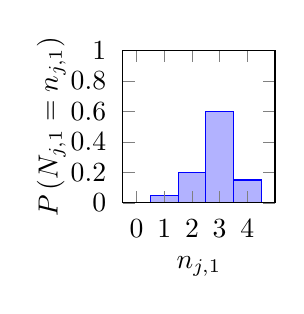
\begin{tikzpicture}
		\begin{axis}[
		width=100,
		height=100,
		domain=0:5,
		area style,
		xmin=-0.5,
		xmax=5,
		ymin=0,
		ymax=1,
		xtick={0,1,2,3,4},
		xticklabel style = {yshift=-0.25em},
		yticklabel style = {xshift=-0.25em},
		xlabel={$n_{j,1}$},
        ylabel={$P\left(N_{j,1} = n_{j,1}\right)$},
        ylabel style={yshift=-0.5em}
		%ylabel near ticks
		]
		\addplot+[ybar interval] plot coordinates {(0.5,0.05) (1.5,0.2) (2.5,0.6) (3.5,0.15) (4.5,0)};
		\end{axis}
		\end{tikzpicture}%
	};
	\node (s2) at (4, 1) {$n_{2,l}=2$}
		edge [<-] node [below right] {Sample} (D2);
	\node (s1) at (4, 3) {$n_{1,l}=3$}
		edge [<-] node [above right] {Sample} (D1);
	\node[draw, fit={(5,1.5) (6,2.5)}, inner sep=0pt, label=center:2, fill=black!20] (T1) {}
		edge [<-] (s1)
		edge [<-] (s2);
	\node[draw, fit={(6,1.5) (7,2.5)}, inner sep=0pt, label=center:1, fill=black!20] (T2) {};
	\node[draw, fit={(7,1.5) (8,2.5)}, inner sep=0pt, label=center:1, fill=black!20] (T3) {};
	\node[draw, fit={(8,1.5) (9,2.5)}, inner sep=0pt, label=center:2, fill=black!20] (T3) {};
	\node[draw, fit={(9,1.5) (10,2.5)}, inner sep=0pt, label=center:1, fill=black!20] (T3) {};
	\node (r) at (6.5, 2.8) {Random order:};
	\node (xl) at (8, 1) {$\boldsymbol{x}^k_{j,l} = [1, 2, 2, 1, M, 2]$};
	\draw [thick,
		decoration={
			brace,
			mirror,
		},
		decorate
		] (8.5, 2.8) -- (9.5,2.8);
	\node[draw, label={Insert maintenance{:}}, fit={(8.5,2.8) (9.5,3.8)}, inner sep=0pt, label=center:M, fill=black!30] (M) {};
	\node (calcp) at (8,-1) {Calculate $p^f_j(\boldsymbol{x}^k_{j,l})$}
		edge [<-] (xl);

	\draw[thick, dotted] (2.5,-1.5) rectangle (11, 4.5)
		node [above left] {Repeat $N$ times, $\bar{p}^f_j = \max p^f_j(\boldsymbol{x}^k_{j,l})${:} };

	\end{tikzpicture}
%\end{document}
